% Chapter 1

\chapter{Background} % Main chapter title

\label{sec:background} % For referencing the chapter elsewhere, use \ref{Chapter1} 

%----------------------------------------------------------------------------------------

% Define some commands to keep the formatting separated from the content 
\newcommand{\keyword}[1]{\textbf{#1}}
\newcommand{\tabhead}[1]{\textbf{#1}}
\newcommand{\code}[1]{\texttt{#1}}
\newcommand{\file}[1]{\texttt{\bfseries#1}}
\newcommand{\option}[1]{\texttt{\itshape#1}}

%----------------------------------------------------------------------------------------

\section{Cost-Effectiveness Models in Healthcare}

\subsection{Objective}
Compare different strategies for detection/treatment of a disease, from health and economic point of view.

\subsection{Methodology}
Simulation model to mimic the strategies and compare the outputs for each strategy to determine which strategies are worth considering. A special ``strategy'' called the natural history describes the progression of the disease without any planned interventions, and it is used to calibrate some the inputs that will be used in the rest of strategies (see section \ref{sec:calibration}).

\begin{figure}[h]
	\centering
	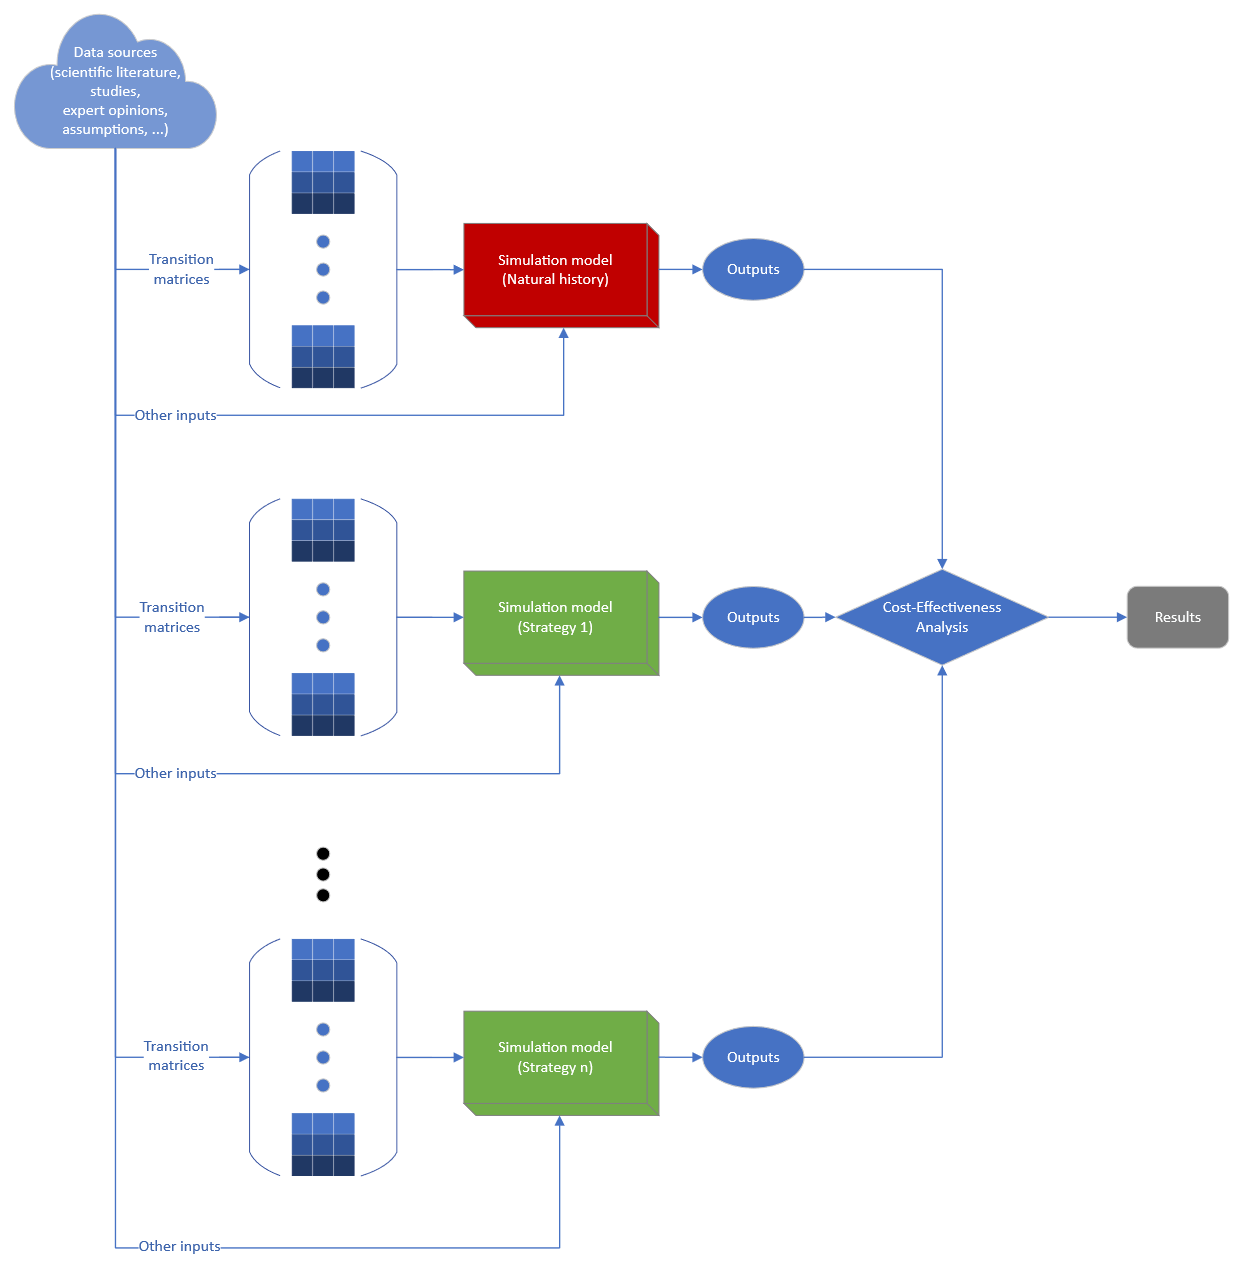
\includegraphics[width=\textwidth]{figures/cea_overview}
	\decoRule
	\caption[CEA overview]{Overview of the cost-effectiveness analysis.}
	\label{fig:cea_overview}
\end{figure}

\subsection{Types of model}
Decision trees, markov model, microsimulation, ... depending on the needs of the domain and the degree of detail and granularity required.

\begin{figure}[h]
	\centering
	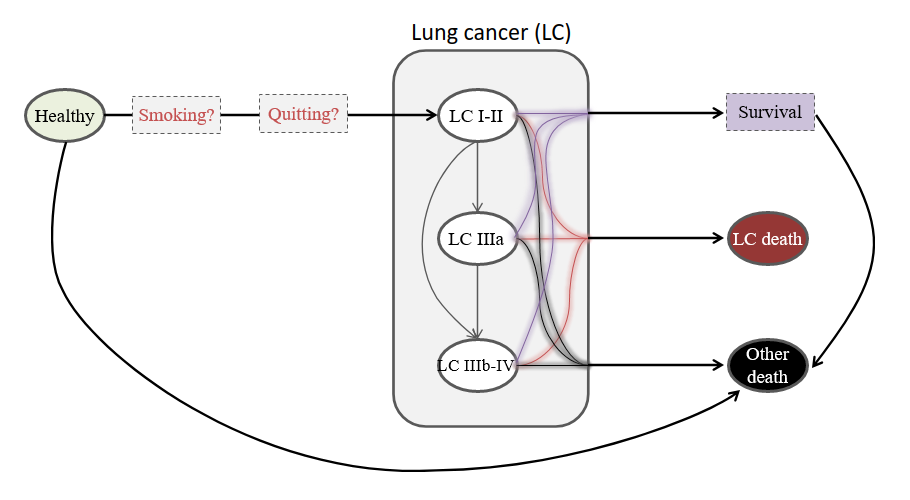
\includegraphics[width=\textwidth]{figures/lung_markov}
	\decoRule
	\caption[Markov state diagram]{Markov state diagram of the lung cancer model.}
	\label{fig:lung_markov}
\end{figure}

\subsection{Inputs}
Parameters extracted from the scientific literature, studies, expert opinions, assumptions, ... An interesting intermediate input are the transition matrices that show the probabilities of transitioning between health states.

\subsection{Outputs}
For each strategy:
\begin{itemize}
\item Effectiveness measure (e.g. Quality-Adjusted Life Years, QALYs)
\item Cost measure (e.g. euros, €)
\item Other general measures of interest: incidence, mortality, ...
\item Other domain-dependent measures: e.g. number of hysterectomies, number of high-grade lesions, ...
\end{itemize}


%----------------------------------------------------------------------------------------

